\subsection{Baza danych}

Baza danych oparta jest o listy programu Sharepoint. \textcolor{pink}{Jak wcześniej wspomniano, nie jest to dedykowane rozwiązanie do budowy takich struktur. }

Na początku należało określić jakie kolumny będą zawierały omawiane listy. W tym celu przeanalizowano pliki z lat poprzednich i wybrano powtarzające się elementy. Pozwoliło to na uzyskanie jednolitego schematu danych:
\begin{itemize}
    \item Service group,
    \item Service main group,
    \item Service sub group,
    \item Business Service (Service Name),
    \item Instruction link,
    \item ID,
    \item Business Service Manager,
    \item Unit Of Measurement,
    \item Settlement Type,
    \item Current Year Plan EUR,
    \item Quantity Current Year,
    \item Next Year Plan EUR,
    \item Quantity Next Year,
    \item Year,
    \item MPK,
    \item Difference,
    \item Indication Number,
    \item Comment Intern,
    \item Comment Date,
    \item Comment Author,
    \item Comment PZ to WOB,
    \item Comment BSM,
    \item Comment K-DES,
    \item Decision,
    \item Final comment.
\end{itemize} 


%%%%%%%%%% Schemat %%%%%%%%%%

        \begin{figure}[h]
            \makebox[0.925\textwidth][c]{
    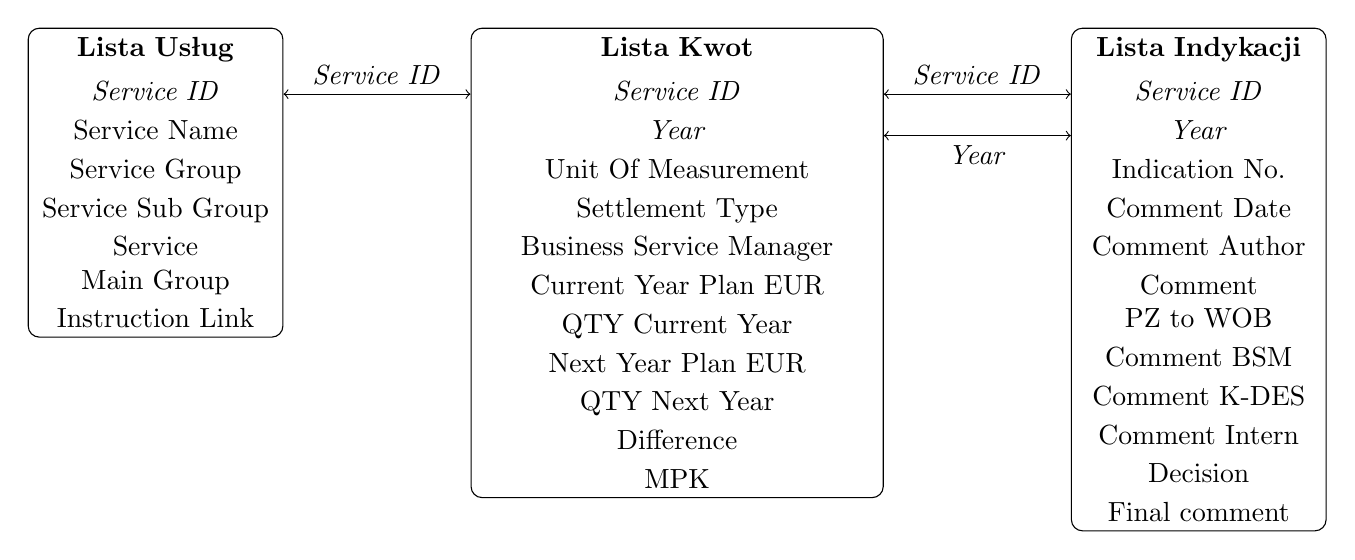
\begin{tikzpicture}
    
    \tikzstyle{ListBlock} = [
        rectangle, 
        rounded corners, 
        minimum width=3cm, 
        minimum height=1cm,
        text centered, 
        draw=black, 
        fill=white,
        anchor=north
    ]
    
    \node (ListaUslug) [ListBlock, text width=3cm] at (0,0) {
      \textbf{Lista Usług}\\[4pt]
      \textit{Service ID}\\[2pt]
      Service Name\\[2pt]
      Service Group\\[2pt]
      Service Sub Group\\[2pt]
      Service Main Group\\[2pt]
      Instruction Link\\[2pt]
    };
    
    \node (ListaKwot) [ListBlock, text width=5cm] 
        at ([xshift=5cm] ListaUslug.north east) {
      \textbf{Lista Kwot}\\[4pt]
      \textit{Service ID}\\[2pt]
      \textit{Year}\\[2pt]
      Unit Of Measurement\\[2pt]
      Settlement Type\\[2pt]
      Business Service Manager\\[2pt]
      Current Year Plan EUR\\[2pt]
      QTY Current Year\\[2pt]
      Next Year Plan EUR\\[2pt]
      QTY Next Year\\[2pt]
      Difference\\[2pt]
      MPK\\[2pt]
    };
    
    \node (ListaIndykacji) [ListBlock, text width=3cm]
        at ([xshift=4cm] ListaKwot.north east) {
      \textbf{Lista Indykacji}\\[4pt]
      \textit{Service ID}\\[2pt]
      \textit{Year}\\[2pt]
      Indication No.\\[2pt]
      Comment Date\\[2pt]
      Comment Author\\[2pt]
      Comment PZ to WOB\\[2pt]
      Comment BSM\\[2pt]
      Comment K-DES\\[2pt]
      Comment Intern\\[2pt]
      Decision\\[2pt]
      Final comment\\[2pt]
    };
    
    \draw [<->] ([yshift=-2em-4pt]ListaUslug.north east) -- node[anchor=south]{\textit{Service ID}} ([yshift=-2em-4pt]ListaKwot.north west);
    \draw [<->] ([yshift=-2em-4pt]ListaKwot.north east) -- node[anchor=south]{\textit{Service ID}} ([yshift=-2em-4pt]ListaIndykacji.north west);
    \draw [<->] ([yshift=-3.5em-4pt]ListaKwot.north east) -- node[anchor=north]{\textit{Year}} ([yshift=-3.5em-4pt]ListaIndykacji.north west);
    
    \end{tikzpicture}}
    \caption{Schemat relacji między listami.}
    \label{SchematList}
\end{figure}
  
%%%%%%%%%%%%%%%%%%%%%%%%%%%%%

Rysunek \ref{SchematList} przedstawia relacje między trzema omawianymi listami oraz sposób powiązania przechowywanych w nich informacji. Podstawę stanowi \emph{lista usług}, która pełni funkcję zbioru danych bazowych o serwisach.

\emph{Lista kwot}, opierając się na identyfikatorze usługi (Service ID), rozszerza model danych o wymiar finansowy, przypisując corocznie aktualizowane wartości do poszczególnych usług. 

\emph{Lista indykacji} natomiast wprowadza dodatkowy poziom szczegółowości, obejmując dane związane z poszczególnymi indykacjami (\english{Indication Number}) -- komentarze, decyzje oraz inne kluczowe informacje.

Takie podejście pozwala na pełne prześledzenie zmian w zakresie kosztów i ilości, a także opinii i ustaleń, bez konieczności powielania danych z Listy usług i Listy kwot. Dzięki temu struktura systemu pozostaje czytelna i zoptymalizowana pod kątem wydajności.

\vspace{1cm}\par
Koncepcja zakładała wykorzystanie relacji pomiędzy listami już na poziomie SharePointa, który umożliwia definiowanie kolumn typu \emph{lookup} do powiązywania dwóch list na podstawie wspólnych elementów w określonych kolumnach. Rozwiązanie to ogranicza się jednak do relacji wyłącznie pomiędzy dwiema listami, co w przypadku konieczności integracji trzech list sprawia, że kolumny typu \emph{lookup} nie mają zastosowania.
\newline
\textcolor{Salmon}{Do implementacji dopisać jak finalnie zrobione są relacje między listami(że na poziomie power apps)}






